% IEEE S&P 2027 submission format.
% Per the CFP: "LaTeX submissions using the IEEE templates must use
% IEEEtran.cls version 1.8b with options 'conference,compsoc'."
% Do NOT add packages/options that change margins, fonts, or line
% spacing (e.g. geometry, usenix): the CFP explicitly flags this as
% grounds for rejection without review.
\documentclass[conference,compsoc]{IEEEtran}

\usepackage{graphicx}
\usepackage{booktabs}
\usepackage{amsmath}
\usepackage{amssymb}
\usepackage{microtype}
\usepackage{xcolor}
\usepackage{caption}
\usepackage{subcaption}
\usepackage{enumitem}
\usepackage{multirow}
\usepackage{hyperref}

% Strip PDF metadata that could deanonymize the submission (author,
% affiliation leaking through document properties rather than the
% visible title page).
\hypersetup{hidelinks,pdfauthor={},pdftitle={Right to Be Forgotten in LLMs: An Empirical Audit of Data Deletion Methods Across Six Platforms},pdfsubject={},pdfkeywords={}}

\title{What Does ‘Delete’ Mean? User Expectations and Observable Data Persistence Across Six LLM Chatbots}

% ANONYMOUS SUBMISSION
% IEEE S&P requires no author names/affiliations on the title page and
% no identity-revealing text in the body (CFP "Anonymous Submission").
% Replace \#XXX with the HotCRP submission number once assigned, and
% swap this block back to the real author list ONLY in the camera-ready
% version after acceptance.
\author{\IEEEauthorblockN{Anonymous Author(s)}
\IEEEauthorblockA{Submission \#XXX}}
% Real authors (restore at camera-ready; do not include in the
% anonymous submission PDF):
% \author{
%   Taiwo Olabamipe \\
%   University of Central Florida \\
%   \texttt{tal17847@ucf.edu}
%   \and
%   Xueqiang Wang \\
%   University of Central Florida \\
%   \texttt{xueqiang.wang@ucf.edu}
%   \and
%   Yao Li \\
%   University of Central Florida \\
%   \texttt{yao.li@ucf.edu}
% }

\begin{document}

\maketitle

% ----------------------------------------------------------------
% TODO(authors): abstract is a summary of the whole paper (motivation,
% method, top findings, implication); write last, once Discussion/
% Conclusion are final. IEEE S&P abstracts run ~150-250 words, plain
% text (no \textit wrapper needed/expected).
\begin{abstract}
TBWL
\end{abstract}
% ----------------------------------------------------------------

\section{Introduction}
\label{sec:intro}

Hundreds of millions of people now share personal, often sensitive,
information with commercial large language model (LLM) chatbots. The
right to erasure under Article 17 of the General Data Protection
Regulation (GDPR) allows individuals, under certain conditions, to
request deletion of personal data concerning them~\cite{gdpr2016}.
Commercial LLM chatbots may retain user data as conversation history,
persistent `memories,'' and conversation content used for model
training. Prior work has shown that LLMs can memorize and later
regurgitate portions of their training data~\cite{carlini2021extracting}.
Yet platforms expose multiple deletion mechanisms, including deleting a
conversation, clearing history, deleting a saved memory, or asking the
chatbot to `forget'' information, whose actual scope is unclear.

Li et al.\ audit the privacy controls exposed by six conversational LLM
platforms and find substantial inconsistencies, including limited support
for deleting individual messages~\cite{li2026privacy}. However, their
analysis focuses on available interface controls rather than whether
invoking those controls on live accounts removes the targeted data.
Related work has documented gaps between user expectations and actual
deletion behavior in search, cloud storage, and website privacy
controls~\cite{bertram2019five,kang2015mydata,ramokapane2017stupid,habib2019empirical},
but whether similar gaps arise in commercial LLM chatbots remains largely
untested.

We therefore examine deletion from both the system and user perspectives:
whether platform controls remove the data they claim to remove, whether
observed behavior aligns with stated policy, what users believe those
controls accomplish, and where these expectations diverge from actual
platform behavior. We ask:

\begin{itemize}[leftmargin=*]
\item[] \textbf{RQ1} (system, behavior): How do commercial LLM chatbots
actually handle data deletion requests?
\item[] \textbf{RQ2} (system, policy gap): Where does observed deletion
behavior contradict each platform's stated policy?
\item[] \textbf{RQ3} (user, expectation & verification): What do users
believe deletion accomplishes, and do they verify that it worked?
\item[] \textbf{RQ4} (user, sensitivity): Does data sensitivity change
deletion method choice, willingness to delete, or expected effort/loss?
\item[] \textbf{RQ5} (divergence): Where does user expectation diverge
most from audited platform behavior, and who bears that gap?
\end{itemize}

To answer these questions, we combine a participatory survey
(RQ3--RQ4) with a technical audit of deletion controls across six
commercial LLM platforms (RQ1--RQ2, RQ5).


\section{Background and Related Work}
\label{sec:background}

\textbf{Right to erasure, at scale.} The GDPR's Article 17 right to
erasure~\cite{gdpr2016} has mostly been studied through its search-engine
delisting mechanism: Bertram et al.\ analyze five years and 3.2 million
URLs submitted to Google for right-to-be-forgotten delisting, finding
requests concentrated on a small number of sites and requesters, and
documenting the operational difficulty of adjudicating erasure at
scale~\cite{bertram2019five}. That line of work audits a single,
well-defined deletion mechanism (search delisting) end to end. Commercial
LLM chatbots instead expose several, informally specified deletion
controls over the same underlying account (conversation-level deletion,
memory-level deletion, natural-language ``forget'' requests, and
account-level deletion), which is the gap this paper's technical audit
(RQ1/RQ2/RQ5) targets.

\textbf{Auditing LLM platform controls.} Closest to this paper, Li et
al.\ walk through the stated access/edit/delete/share
controls of six conversational LLM platforms (a partially overlapping
set with the six audited here; see \S\ref{sec:intro}) and find them inconsistently
implemented, with most platforms not supporting deletion of an individual
message~\cite{li2026privacy}. That audit characterizes what controls each
platform's interface exposes; it stops short of testing, on live
accounts, whether invoking a given control actually removes the data it
names (the system-side gap RQ1/RQ2 target), and it does not survey users
about those controls. This paper's technical audit and participatory
survey close these two gaps respectively.

\textbf{Machine unlearning.} A deletion request that only removes a
record from a database does not, by itself, remove that record's
influence on a model already trained on it. Bourtoule et al.\ formalize
this distinction and propose \textit{SISA} training to make exact
unlearning practical, framing verifiable removal of a data point's
influence as a distinct technical problem from simply deleting the
underlying record~\cite{bourtoule2021machine}.

\textbf{User mental models of deletion.} Usable-privacy research has
repeatedly found that people's mental models of ``deletion'' do not
match how deletion is actually implemented. Kang et al.\ show that many
users hold incomplete or inaccurate models of how the internet handles
their data generally, with direct consequences for the privacy decisions
they make~\cite{kang2015mydata}. Ramokapane et al.\ study cloud-storage
deletion specifically and find users often cannot tell whether a delete
action removed data locally, from the cloud, or from other synced
devices, and adopt ad hoc coping strategies (e.g., deleting the same
item multiple times) in response to that uncertainty~\cite{ramokapane2017stupid}.
Habib et al.\ audit the deletion and opt-out controls of 150 websites
directly and find that even when a control exists, it is often
inconsistently located, under-explained, or effectively non-functional --
an interface-level failure mode distinct from, but compounding, any
backend failure to actually delete data~\cite{habib2019empirical}.

\textbf{LLM memory specifically.} On the user side specifically, Zhang
et al.\ interview 18 users of LLM chatbots with retrieval-augmented-
generation-based ``memory'' features and find diverse, often incomplete
mental models of what the memory stores and how it is used, alongside an
explicit desire for finer-grained control over reviewing, editing, and
deleting individual memories~\cite{zhang2025understanding}.

\textbf{Positioning.} Li et al.\ show that LLM platforms' stated
deletion controls are inconsistent by design~\cite{li2026privacy}; no
identified prior work tests whether those (or comparable) controls
work as stated on live accounts, or pairs such a test with a matched
participant survey of what the same controls are believed and used to
accomplish. This paper reports both halves of that pairing: a technical
audit of whether six commercial platforms' deletion controls remove the
data they claim to (RQ1, RQ2), and a participatory survey of which
deletion methods people actually choose, how those choices and their
perceived cost/protection change with data sensitivity, and where
expectation and verification behavior part ways with what the methods
are actually likely to do (RQ3, RQ4;
\S\ref{sec:sample-knowledge}), which allows the two to be compared directly
against each other (RQ5).

\section{Methodology}
\label{sec:methodology}

\subsection{Participatory Survey}
\label{sec:survey-methodology}

The survey was built and administered in Qualtrics, and respondents were
recruited through Prolific (recruitment, consent and compensation are
described in the Ethics Considerations section). We set no formal sample-size
target or power calculation and aimed for roughly 200 respondents. It uses a within-subject design: the same participants rate two
scenario blocks in a fixed order, always the less-sensitive
data-deletion vignette before the more-sensitive one, each repeating an
identical question battery. Order was not counterbalanced, so scenario
(data sensitivity) and presentation order are perfectly confounded in
this dataset; \S\ref{sec:sensitivity-effect} and \S\ref{sec:limitations}
report the resulting scenario-level differences as observed, not as an
isolated effect of sensitivity. Each scenario battery includes
three multi-item Likert scales (perceived protection with 5 items, effort
with 4 items, and benefit loss with 3 items) plus single-item measures of
deletion method choice, willingness to delete, deletion expectations, and
verification behavior. All six scale-by-scenario combinations meet
conventional reliability thresholds (Cronbach's $\alpha=0.87$--$0.92$),
confirmed identically by both analysis pipelines described in
\S\ref{sec:sample-knowledge}.

\textbf{Scenarios and attention checks.} Each scenario is a short
chatbot conversation followed by the instruction to imagine deleting the
location data disclosed in it. The less-sensitive scenario is a weather
query: the user gives a city and asks whether to bring an umbrella. The
more-sensitive scenario is a health query: the user gives a home address
and asks for the nearest clinic for treatment of a sexually transmitted
infection. Two instructed-response items check attention (``Please select
`Sometimes' for this question'' and ``Please select `Agree' for this
question''). The full scenarios and scale items are in Appendix~\ref{sec:instrument}.

\textbf{Missingness and aggregation.} Of 235 raw Qualtrics submissions,
17 incomplete/abandoned attempts are excluded first, leaving 218; 1
further response is dropped for failing an attention check (a missing,
unanswered check item is not treated as a failure), and 36 for reporting
they had never deleted chatbot data, leaving 181 eligible.
Within that eligible set, three overlapping bases are used depending on
the analysis: \textit{less} and \textit{more} (respondents who answered
that scenario's method-choice item, used for between-method comparisons
within a single scenario) and \textit{paired}, $n=177$ (respondents who
answered both, used for every within-subject less-vs-more comparison).
Pooled-across-scenario analyses (e.g.\ Table~\ref{tab:contingency}) treat
each participant's response in each scenario as its own observation (352
observations from the 176 participants who named a method in both
scenarios) and account for the repeated measures by clustering on
participant, as described under Statistical analysis below. Headline paired mean differences
(willingness, protection, effort, benefit loss) are reported with 95\%
confidence intervals from a percentile bootstrap (10,000 resamples,
seeded for reproducibility) over the paired-respondent differences, since
the Wilcoxon signed-rank test used for these comparisons (chosen over a
paired $t$-test per a per-scale Shapiro-Wilk normality check on the
difference scores) has no closed-form interval for the mean difference
itself.

\textbf{Sample scope.} The eligibility screen keeps only respondents who
had deleted chatbot data at least once, so every survey result describes
people who found and used some deletion control. The results are silent on
the 36 of 218 complete respondents (16.5\%) who had never deleted chatbot
data, a group that may face the largest barriers to discovering deletion
controls at all.

\textbf{Statistical analysis.} Table~\ref{tab:analysis-families} lists each
inferential analysis, its test, and the family over which Holm's step-down
correction was applied. Holm-adjusted values are reported as
$p_{\mathrm{Holm}}$ and unadjusted values as $p$; a single claim never
mixes the two. We treat every survey analysis as exploratory, so $p$-values
describe the strength of evidence within a family, not a paper-wide error
rate. A nonsignificant result is read as ``no association detected,'' with
the estimate and its uncertainty where available, not as evidence of no
association: the smallest qualifying method groups contain 14 participants,
so the tests have limited power to detect small differences. Only methods
chosen by at least 14 distinct participants enter inferential tests. Fisher
exact tests on two-column tables (method by selected or not) are computed by
exact enumeration, so every reported $p$-value is reproducible.

Pooled analyses (both scenarios combined) fit a generalized estimating
equation (GEE) with participant as the cluster, deletion method and scenario
as predictors, an independence working correlation, and robust (sandwich)
standard errors. The omnibus test is a Wald test that all method terms are
zero. Rating scales use an identity link and 0/1 expectation indicators a
logit link; an option that no participant chose in some method group cannot be
estimated with the logit link and enters its Holm family at $p=1$. The
independence working correlation keeps the point estimates equal to the
observed group means, which matters because method varies within a
participant (participants who switched methods appear in several groups) and
a non-independence working correlation is consistent only under stronger
assumptions about that variation. Sensitivity analyses used an exchangeable
working correlation and, for the indicators, a linear-probability model.
Post hoc contrasts compare all pairs of methods and are run only where the
Holm-adjusted omnibus test is significant.

\begin{table*}[t]
\centering
\caption{Inferential Survey Analyses, Tests, and Holm Correction Families}
\label{tab:analysis-families}
\small
\begin{tabular}{@{}p{0.29\textwidth}p{0.37\textwidth}p{0.28\textwidth}@{}}
\toprule
Analysis & Test & Holm family \\
\midrule
Scenario shift in protection, effort, benefit loss (paired, $n=177$)
  & Wilcoxon signed-rank, or paired $t$ where the difference scores pass Shapiro-Wilk
  & 3 scales \\
Scenario shift in willingness (paired)
  & Wilcoxon signed-rank
  & Single test, unadjusted \\
Scenario shift in option selection (expectation, verification)
  & McNemar test per option
  & Options within each item (7, 8) \\
Method choice shift between scenarios
  & Stuart-Maxwell omnibus; McNemar test per method
  & 7 methods \\
Ratings by method, within a scenario
  & Kruskal-Wallis; Dunn's post hoc
  & Omnibus tests unadjusted; pairs within Dunn's test \\
Ratings by method, pooled
  & Participant-clustered GEE (Wald); pairwise contrasts
  & 3 scales; 6 method pairs \\
Expectation and verification by method, within a scenario
  & Chi-square, or $r\times c$ Fisher exact when expected counts are below 5
  & Options within each item and scenario (7, 8) \\
Expectation by method, pooled
  & Participant-clustered logit GEE (Wald)
  & 7 options \\
Ideal methods, between scenarios
  & McNemar exact test per method
  & 8 methods \\
Ratings by method, between scenarios
  & Mann-Whitney $U$ per method
  & 4 methods within each scale \\
Ratings on participant characteristics
  & Ordinary least squares, participant-clustered standard errors
  & Unadjusted \\
Measurement model
  & Exploratory factor analysis (principal axis, oblimin), parallel analysis
  & Not applicable \\
\bottomrule
\end{tabular}
\end{table*}

\subsection{Deletion-Request Prompt Corpus}
\label{sec:prompt-corpus}

One arm of the technical audit (\S\ref{sec:audit-methodology}) types real
deletion requests into each platform rather than researcher-authored
phrasings. Those requests originate in the same instrument described in
\S\ref{sec:survey-methodology}: after selecting a deletion method within
each scenario block, participants typed the exact message they would send
the assistant to carry it out and stated their rationale for that
phrasing. Across both scenario blocks this yielded 415 raw responses from
209 participants; after removing blank/unusable entries and within- and
cross-participant duplicates, 375 distinct prompts remained. This corpus
was extracted from an earlier raw survey export (217 rows, dated
2026-07-27, read without a completion-status filter) than the one the
quantitative survey results (\S\ref{sec:sample-knowledge}) are drawn from
(235 rows, dated 2026-09-09, of which 218 are complete submissions);
209 of 217 in that earlier export left a non-blank prompt in at least one
scenario. The two exports differ in both collection date and completeness
filtering, so they are not directly arithmetic-comparable snapshots of an
identical pipeline. Corpus construction does not apply the eligibility
screen described in \S\ref{sec:sample-knowledge} (attention check,
prior-deletion-experience filter): a prompt is included whenever its
author wrote one, independent of whether that respondent later qualified
for the survey's own analysis sample, so the corpus's 209/375 figures and
the survey's 181-eligible/177-paired figures are two different
denominators over two separately-filtered raw pools, not two measurements
of the same population. Each was
scrubbed of residual personally identifying text (32 of 375 prompts
altered: 20 organization-name, 12 location-name, and 3 person-name
redactions) and passed through an
automated feature-extraction step labeling candidate dimensions including
a coarse deletion-location category, used only to stratify the sampling
step below, not as the reliability-bearing codes reported next.

\textbf{Coding and reliability.} Two coders hand-coded prompts against a
seven-dimension codebook: deletion location (the storage surface the
request names: the current conversation, the assistant's persistent
memory, the account as a whole, a named backend or database, or a
forward-looking ``stop using this'' instruction that names no location),
justification, data type (\emph{what}), grammatical mood, tone, verb
register, and any accompanying secondary request (for example, asking for
confirmation, or asking the assistant to preserve everything else the
deletion target excludes). Each dimension was coded on 50 items.
Inter-rater reliability was computed with Gwet's $AC_1$~\cite{gwet2008ac1}
rather than Cohen's $\kappa$: several dimensions have highly skewed
category distributions (one label covering 88--96\% of items), under which
$\kappa$'s chance-agreement term is known to understate true
agreement~\cite{gwet2008ac1,wongpakaran2013comparison}.
Table~\ref{tab:ac1} reports these values. Each of the two coders labeled a
50-item sample independently, without seeing the other's codes.

The deletion-location definition was refined after piloting, and its
reliability is reported on a sample coded under the final definition. A
location counts only when the prompt names it with an explicit referent
(conversation or chat, memory, account, or a database, server, or
training data); quantifiers such as ``all'' and generic containers such
as ``history'' or ``messages'' do not qualify. When a prompt names
several locations, a named database governs over a conversation or
memory, and a forward-looking clause governs over a named conversation.

\begin{table}[t]
\centering
\caption{Inter-Rater Reliability, $n=50$ per Dimension}
\label{tab:ac1}
\small
\begin{tabular}{lccc}
\toprule
Dimension & Agreement & \% & Gwet's $AC_1$ \\
\midrule
Deletion location$^{\dagger}$ & 44/50 & 88.0 & 0.862 \\
Justification           & 47/50 & 94.0 & 0.931 \\
What (data type)        & 43/50 & 86.0 & 0.826 \\
Mood                     & 48/50 & 96.0 & 0.955 \\
Tone                     & 43/50 & 86.0 & 0.807 \\
Verb register            & 47/50 & 94.0 & 0.938 \\
Accompanying request     & 46/50 & 92.0 & 0.917 \\
\midrule
Pooled (350 ratings) & 318/350 & 90.9 & 0.905 \\
\bottomrule
\end{tabular}
\vspace{4pt}

\footnotesize{$^{\dagger}$Coded under the final definition (see text).}
\end{table}

\textbf{Sampling for the technical audit.} A 138-item sample was drawn
from the 375-item corpus by proportional stratified sampling on the
automated deletion-location label (a floor was applied so that
low-frequency categories were not eliminated from the draw), for use
verbatim as the chat-typed erasure request in the technical audit's
NL-forget-prompt cells (\S\ref{sec:audit-methodology}). The sample is a fixed item list, not regenerable under a different random seed.

\subsection{Technical Audit}
\label{sec:audit-methodology}

The technical audit is a black-box behavioral test of six commercial LLM
chatbot platforms' consumer-facing deletion controls (Claude, ChatGPT,
Gemini, Copilot, Perplexity, and DeepSeek), conducted against each
platform's live web interface rather than its API, since the API does
not expose the memory, settings, and deletion surfaces the study's
research questions concern. Each platform is tested through a
researcher-controlled account under browser automation
(Playwright)\footnote{Two of the six platforms additionally require a
stealth plugin to pass Cloudflare bot-detection checks that otherwise
block any automation-driven session; see the Ethics Considerations
section.}, driven by an orchestrator that loads each test cell's
parameters from a pre-registered experiment design and dispatches it to
the matching platform-specific implementation.

\textbf{Design.} A \textit{cell} pairs one injection method with one
erasure method on one platform. Three injection methods test distinct
memory-formation pathways: \textit{I1}, an offhand conversational mention
with no explicit request to remember it, testing whether a platform
infers memory-worthiness on its own; \textit{I2}, an explicit
``please remember'' instruction in conversation; and \textit{I3}, a
direct entry into a platform's memory/settings field where one exists. A
fourth condition, \textit{FILE}, tests document-based disclosure by
uploading a PDF containing the same disclosure content instead of typing
it. Erasure methods are drawn from each platform's own available
controls and range from conversation-level deletion, through per-item and
bulk memory deletion, to account- or privacy-dashboard-level erasure,
reflecting that no two platforms expose an identical set of deletion
surfaces. The full design comprises 85 cells: 73 platform/injection/
erasure combinations plus 12 file-upload cells, distributed unevenly
across platforms in proportion to how many memory and deletion surfaces
each one actually exposes. Three further ChatGPT cells (per-item memory
deletion crossed with I1, I2, and I3) were removed before any run, because
ChatGPT's redesigned memory interface no longer offers that action; they
are not counted.

\textbf{Policy commitments.} For RQ2, each cell in the 85-cell battery is
assigned a \textit{commitment type}, set only from what the platform's own
published documentation says about the erasure action applied to that
cell's injection surface. The source URL and the quoted language are
recorded per cell. \textsc{Deletes} means the documentation states that
the action removes the content. \textsc{Does not delete} means it states
that the action does not reach the content, as in ``deleting a
conversation does not delete saved memories''; this is a statement of
scope, not a promise that the content stays recoverable, so removal
beyond it is not a contradiction. \textsc{No commitment} means the
documentation is silent on the action for that surface, so any expectation
would be an architectural inference rather than a documented promise.
\textsc{Unrelated} means the erasure mechanism and the injection surface
are architecturally separate, so the cell tests neither.
\textsc{Not testable} means the surface cannot be reached on the test
account. Only the first two types can support a verdict on policy; cells
of the other three are reported descriptively. The verdict itself is
derived from the measured outcome by the rule in
Table~\ref{tab:consistency-rule}, not judged case by case. One documented
exception applies to requests typed into the chat to forget a fact. Where
a platform's documentation says such a request removes the saved memory but
leaves mentions of the fact in past conversations, a token recovered only
from the conversation where the fact was first disclosed is reported as
recovered but is not counted as contradicting the commitment.

\textbf{NL-forget-prompt extension.} The 138 participant-written erasure
requests sampled in \S\ref{sec:prompt-corpus} form an additional set of
cells appended to the 85-cell design: one cell per prompt per platform
(138 prompts $\times$ 6 platforms). Each prompt is typed verbatim as the
erasure request, with only its disclosed referent substituted in, after a
fixed I1 (offhand conversational) disclosure. Injection type is held
constant so that erasure phrasing is the only varying factor, and recall
uses the same three-probe design (R1/R2/R3) as the 85-cell battery. All
cells on a platform share one dedicated account, distinct from the
battery's accounts, with attribution secured by each cell's unique
referent and token. This assumes that an erasure request does not erase
another cell's content, so a prompt is excluded if its wording has a high
probability of doing so. Five prompts meet this criterion: each asks for
all of the user's data, or all data in the chat, without naming a
referent. The remaining 133 each name a single referent, so their wording
does not ask for any other cell's content to be erased. They are run,
giving 798 cells (133 prompts $\times$ 6 platforms).

\textbf{Contamination control.} Accounts are reused across cells rather
than provisioned fresh per cell; attribution across cells sharing an
account is instead secured by giving every cell a unique \textit{referent}
(the conversational topic disclosed, e.g. a hobby or habit) and a unique
\textit{token} (a distinctive codename attached to that referent, 2--4
words, drawn to give each token a quantifiable, individually low guess
probability, following the canary-design rationale of prior work on
measuring unintended memorization~\cite{carlini2019secret}). A recall
probe that surfaces a cell's token is attributable to that cell alone.
Disclosure content is restricted by a narrow exclusion list (weapons,
drugs, sexual content, profanity, and a slur/explicit-term denylist)
chosen to avoid triggering platform content filters without otherwise
constraining topic naturalism.

Token uniqueness alone is not sufficient where a cell's own erasure
action is not scoped to that cell's referent at all: an account-wide or
``clear everything'' action reaches every other cell sharing that
account regardless of referent. Two further account-provisioning rules
address this. First, within the 85-cell battery, any cell whose erasure
action shares an account with a sibling cell testing the same
account-wide surface, or with a cell still inside its 31-day post-erasure
recall window, is moved to its own dedicated account before either cell
runs, so that a ``confirmed erased'' or ``not found'' recall outcome can
be attributed to the mechanism under test rather than an unrelated
blanket action that happened to share its account. Second, cross-platform
account reuse does not require this isolation: the same login credential
is deliberately reused across multiple platforms because each platform's
memory and conversation history is siloed to its own backend, confirmed
directly in this study: an account-wide erasure action executed on one
platform had no observed reach into a different platform sharing the
same login credential. For the NL-forget-prompt extension specifically,
each platform's cells share a single dedicated account (distinct from
the 85-cell battery's accounts) rather than one account per cell, since
per-cell token uniqueness is sufficient for the 133 of 138 prompts that
each name a single referent. The remaining 5 prompts ask for all of the
user's data without naming a referent, so each has a high probability of
erasing every other prompt's still-untested content on the shared
account. They are excluded (30 of the 828 cells) rather than isolated on
dedicated accounts.

Provisioning by request scope is a necessary but not sufficient
safeguard on its own, since a request's wording can understate its
actual operational reach. Scheduling adds a second, independent layer:
within any account, every due erasure is additionally ranked by a
text-match against a fixed list of broad-action keywords (``clear
all,'' ``delete all,'' ``bulk,'' ``privacy dashboard,'' and equivalent
phrasing), and cells sharing an account are always run narrowest-ranked
first, broadest-ranked last, so a broad action cannot execute before a
narrower sibling cell still awaiting its own turn on the same account.
This scheduling safeguard was added after a real instance of the failure
it now prevents: a broad erasure run manually before this ordering
existed wiped three still-pending narrower cells sharing its account,
which were subsequently re-injected. It is deliberately redundant with,
not a replacement for, the static per-cell account isolation described
above.

\textbf{Temporal design.} Each cell runs as three separately scheduled
events rather than in immediate succession: erasure occurs 48 hours
after injection, and recall occurs 31 days after erasure. This window is
sourced from the platforms' own stated data-deletion completion
commitments, not an arbitrary delay. Recall is tested two ways within
that single 31-day-post-erasure phase: \textit{same-session} (probing
within one continuous browser session) and \textit{cross-session} (a
separate session against the same account), both run back to back rather
than at separately staggered times.

\textbf{Recall probes.} Three probe types run at each recall point.
\textit{R1} (direct) always asks two open questions about the disclosed
referent, worded differently, the second a natural same-conversation
follow-up run regardless of what the first reply contained. R1 has no
forced-choice stage. Ranking the true value against counterfactuals, as
prior work on quantifying personal-data memorization does, relies on
model likelihoods~\cite{staufer2025wikimem}, which consumer chat
platforms do not expose. A closed question listing candidate tokens would
instead have to type the correct token into the account being tested, on
the same conversational surface I1 injection uses to plant a disclosure,
and would leave a one-in-four chance of a correct answer by guessing
alone. Recall is therefore probed by open questions only. Asking each
open probe twice, in different wordings, reflects that model output can
change with superficial features of a prompt~\cite{sclar2024quantifying}.
Probing goes through each platform's consumer web interface, with the
question asked in a new conversation after the information was given
earlier, as in the evaluation of commercial chat assistants in
LongMemEval~\cite{wu2025longmemeval}.
\textit{R2} (settings) directly inspects the platform's own
memory-listing interface where one exists. \textit{R3} (indirect) always
sends two unrelated tasks that never mention the token, the second again
regardless of what the first produced, testing whether the disclosed
content leaks into unrelated generation rather than only being
recoverable when directly asked about. Running two attempts unconditionally,
for both R1 and R3, rather than only following up when the
first result is surprising, is a deliberate fix to the outcome-dependent
repetition asymmetry discussed under ``Outcome recording and repetition''
below: every cell gets the same number of checks, not just the ones whose
first answer departed from what the documentation predicted. R1 and R3
responses are matched against the token without regard to case, with
hyphens, underscores and whitespace treated as equivalent (so
``Nutcase-Taps'' matches ``Nutcase Taps'') and the token required to
appear as whole words. A reply is scored automatically only when it
contains the full token in a sentence with no negation, refusal or
question cue. A reply that contains only some of the token's words, or
contains the full token only in sentences with such a cue (for example
``I don't have any record of Nutcase Taps''), is held for human review
and coded FOUND, NOT FOUND or UNCLEAR, with UNCLEAR cases going to a
second reviewer; for R2, the reviewer records whether the fact appears
verbatim, paraphrased or not at all. The cue check only routes replies to
a person and never decides an outcome.

Within each recall visit the probes run in a fixed order, R2, then R3,
then R1, the order set in the pre-registered design. The order limits
contamination between probes: R2 only reads a page and adds nothing to
the account, R3 runs before any direct question can put the token back
into the account, and R1, which names the referent outright, runs last.
This follows the finding from human memory research that taking a
retrieval test strengthens later retention of what was tested~\cite{roediger2006test},
which we treat as an analogy for a chat account's history and memory, not
as evidence about these platforms. R1 and R3 likewise mirror the
distinction between explicit and implicit tests of memory~\cite{graf1985implicit}:
R1 asks for the disclosure outright, and R3 looks for its influence on an
unrelated task. One related limitation remains and is discussed in
\S\ref{sec:limitations}: this design has no never-injected negative-control
or injected-but-not-deleted positive-control cells.

The two visits are not independent, because the cross-session visit runs on
an account the same-session visit has already written to. If a
same-session reply contains the token, that reply enters the account's chat
history and may be saved as a memory, so a cross-session leak could be an
echo of the first visit rather than evidence about the original data. We do
not delete the probe conversations between visits: deletion is the
behavior under test, is unreliable on these platforms, and would add an
unverified second erasure to every cell. Instead, the same-session visit is
the primary measurement, since it is the only one that runs on an account
no probe has touched. A cross-session result is coded as independent only
when no same-session R1 or R3 reply contained the full token, including
replies that named it with a negation or question cue, since those also type
the token into the chat. When one did, a cross-session leak is coded as a
repeat that is not independent. Each recall also records whether the
memory page showed the token at the second visit but not at the first, which
would indicate that our own probes wrote it. Because R2 runs before any chat
in a visit, the first visit's R2 is a baseline that no probe has touched.
% TODO(authors): also report (a) a spot check of a random sample of automatically accepted
% FOUND replies, since a negation worded outside the cue list would be
% accepted, and (b) agreement between the two reviewers on a
% double-reviewed sample (Gwet's AC1).

\textbf{Measurement scope.} This design measures what a platform says and
what remains observable, not what its storage holds. Each cell yields four
measurements (``Outcome recording and repetition'' below): the
acknowledgment in the platform's reply, whether the interface visibly
changed after the erasure action, whether the content is recoverable at
the 31-day recall point, and whether the outcome is consistent with the
platform's documented commitment. Recoverability is read from three
probes: whether the content still appears in a platform's own
memory-listing interface (R2), whether it resurfaces unprompted in
unrelated generation (R3), and whether it is recoverable when directly
asked (R1). None of these observations establishes or
rules out removal from backend storage, training datasets, or an
already-trained model's parameters: a ``token not found'' outcome shows
the token did not surface through the probes tested, not that the
underlying data was deleted from every system that might hold it, and a
``token found'' outcome shows the content remained recoverable through at
least one tested surface, not which storage location supplied it. The
canary-style token design above supports attributing a recovered token to
its originating cell~\cite{carlini2019secret}; it does not convert a
non-recovery into evidence of erasure. RQ1 and RQ2 are accordingly scoped
throughout this paper to platform-observable behavior and consistency with
documented commitments, not to backend or training-data erasure, which
this design cannot verify.

\textbf{Outcome recording and repetition.} Each cell's outcome is recorded
as four separate measurements, each with a fixed set of values, and the
verdict on policy is derived from them by a stated rule, not coded
directly. \textit{Acknowledgment} is what the platform's reply says about
the erasure request: complied, partial, refused, deflected, silently
ignored, asked to connect an app (see ``Platform changes'' below), or no reply for actions performed through the interface, which
produce none. It shows what the platform said, not that anything was
deleted. \textit{Interface change} is whether the intended surface
visibly changed after the action (changed, unchanged, or not
observable), coded from the post-erasure screenshot.
\textit{Recoverability} is the recall outcome (``Recall probes'' above):
recovered by at least one probe, not recovered, or indeterminate when the
injection check did not establish that the platform had retained the
content, so that a missing token is never read as evidence of deletion.
\textit{Policy consistency} combines the cell's commitment type with the
interface change and recoverability by the rules in
Table~\ref{tab:consistency-rule}. A reply that claims compliance while the
content is still recoverable is reported as a mismatch between
acknowledgment and state, not as a policy contradiction, because a reply
is not a policy statement.

\textbf{Retention at injection.} A missing token counts as evidence of
deletion only if the platform kept the fact before the erasure. Running an
extra, un-erased copy of every cell to check this would double the number
of cells, so we read it from what the platform showed when the fact was
given, in the saved transcript and the screenshot. Each cell gets one of
five values. \textit{Shown} means the interface itself displayed a memory
notice (for example ``Memory updated''). \textit{Claimed} means the reply
says, in so many words, that it saved the fact or will remember it.
\textit{Denied} means the reply says it cannot store it (``I can't save
new memories right now''). \textit{Acknowledged} means the reply only
reacted to the fact (``Noted!'') without saying it was stored. \textit{No
signal} means neither the reply nor the screen mentioned storage. Only
shown and claimed cells establish that the fact was kept. For every other
value, a token that is not recovered is reported as inconclusive, not as
evidence of deletion, and only denied points to the fact not having been
kept. Some interfaces draw the notice outside the reply text, so it is
missing from the saved transcript and is read from the screenshot instead.
A missing notice is not read as ``not stored'', because it can appear after
the screenshot is taken. Cells that upload a file are left out, since they
are classified separately.

\begin{table}[t]
\centering
\caption{How policy consistency is derived. The commitment type fixes
which combinations of interface change and recoverability count as
consistent or contradicted. Cells of the last three types are never
contradicted, so they are reported descriptively.}
\label{tab:consistency-rule}
\small
\setlength{\tabcolsep}{3.5pt}
\begin{tabular}{@{}p{0.23\columnwidth}p{0.25\columnwidth}p{0.27\columnwidth}p{0.15\columnwidth}@{}}
\toprule
Commitment type & Contradicted & Consistent & Indeterminate \\
\midrule
\textsc{Deletes} & recovered, or interface unchanged
 & not recovered, and interface not unchanged & otherwise \\
\textsc{Does not delete} & never & recovered & not recovered \\
\textsc{No commitment}, \textsc{Unrelated}, \textsc{Not testable}
 & never & never & always \\
\bottomrule
\end{tabular}
\end{table}

Acknowledgment is recorded from the platform's single response to the
erasure request; there is no safe way to ask a platform to comply with the
same erasure request a second time without either repeating an
already-completed action or changing what is being measured. For the
chat-based erasure requests the reply text was not saved during the run,
so it was read from the post-erasure screenshot by optical character
recognition (macOS Vision, language correction disabled). A reply counts
as complete only when both its start and its end are visible on screen; a
reply that was cut off by the edge of the window, covered by an overlay, or
not yet displayed when the screenshot was taken is reported as not
captured.
% TODO(authors): if the incomplete replies are later recovered from the
% platforms' stored conversations, say so here and report the counts
% (complete / not captured) with the audit results.
Recall, by contrast, now uses a fixed
two-attempt policy applied identically to every cell regardless of
outcome (``Recall probes'' above): R1 and R3 each run twice,
unconditionally, rather than only receiving a follow-up when the first
attempt's result was surprising. This replaces an earlier design that
reran a cell's recall only when its observed outcome departed from what
the platform's documentation predicted (``Policy commitments'' above),
which held expected and unexpected recall outcomes to
different evidentiary standards; that asymmetry no longer applies to
recall, since every cell now gets the same two-attempt check independent
of what either attempt finds. Results (\S\ref{sec:audit-results}) report
both attempts for every cell, not just a single collapsed outcome. Every
phase of every cell (injection, erasure, same-session recall,
cross-session recall) saves a transcript and a screenshot of the browser
window, retained per platform and cell for independent review. All six accounts
are provisioned on each platform's free, no-cost tier; where a platform
gates a tested surface behind a paid tier, that is recorded as a result
rather than treated as a methodology gap. File-upload cells (\textit{FILE})
use a distinct, more granular verification taxonomy reflecting that a
document can be read into a conversation, into persistent memory, into
both, or into neither without a follow-up request. Extraction is
checked passively first (does the platform's own unprompted reply or
memory listing surface the token) and, only if neither does, once more
after an explicit follow-up request to summarize the document.

\textbf{Platform changes.} Copilot moved from \texttt{copilot.microsoft.com}
to \texttt{copilot.com} during the study, so its recall runs on an interface
that differs from the one used at injection (\S\ref{sec:limitations}). On
Gemini, 7 of 133 chat-based erasure requests received a prompt to connect
Google Keep instead of a reply. Nothing was deleted, and we code these as a
separate acknowledgment value (asked to connect an app), not as compliance
or refusal.

\section{User Study}
\label{sec:sample-knowledge}

Of 218 complete responses, 181 passed the attention and eligibility checks, and 177 answered both scenarios; these 177 participants form the analysis sample (Table~\ref{tab:demographics}). They were young (73\% under 45), 58.8\% men and 40.7\% women, and educated (62.1\% held at least a bachelor's degree). All had used at least one of the six chatbots: ChatGPT (99.4\%) and Gemini (92.7\%) were nearly universal, Claude and Copilot were each used by 67.8\%, and Perplexity and DeepSeek were the least used and most recently adopted (Figure~\ref{fig:ai-tenure}). Privacy knowledge was high (mean 5.06 of 6 correct; 46.3\% answered all six correctly), as were self-rated AI literacy (mean 3.83 of 5) and concern about submitting personal information to chatbots (mean 3.80 of 5). Participants most often shared general questions (84.7\%), preferences or opinions (63.8\%) and work information (54.2\%) with chatbots, and 36.7\% shared health information and 27.7\% location information. The data they had tried to delete were spread across these types: preferences or opinions (40.1\%), general questions (39.0\%), work information (32.2\%), health information (28.8\%) and sensitive personal experiences (26.6\%).

\begin{table}[t]
\centering
\caption{Sample demographics ($n=177$).}
\label{tab:demographics}
\small
\setlength{\tabcolsep}{3.5pt}
\begin{tabular}{llcc}
\toprule
Variable & Response & $n$ & \% \\
\midrule
\multirow{6}{*}{Age}
 & 25--34 & 56 & 31.6 \\
 & 35--44 & 45 & 25.4 \\
 & 18--24 & 29 & 16.4 \\
 & 45--54 & 27 & 15.3 \\
 & 55--64 & 17 & 9.6 \\
 & 65+    & 3  & 1.7 \\
\midrule
\multirow{3}{*}{Gender}
 & Man               & 104 & 58.8 \\
 & Woman             & 72  & 40.7 \\
 & Prefer not to say & 1   & 0.6 \\
\midrule
\multirow{6}{*}{Education}
 & Bachelor's degree      & 75 & 42.4 \\
 & Graduate/professional  & 35 & 19.8 \\
 & Some college, no degree & 30 & 16.9 \\
 & Associate's/technical  & 19 & 10.7 \\
 & High school/GED        & 15 & 8.5 \\
 & Some high school or less & 3 & 1.7 \\
\midrule
Privacy Knowledge (0--6) & $M=5.06$, $Mdn=5.0$ & n/a & n/a \\
\bottomrule
\end{tabular}
\end{table}

\begin{figure}[t]
\centering
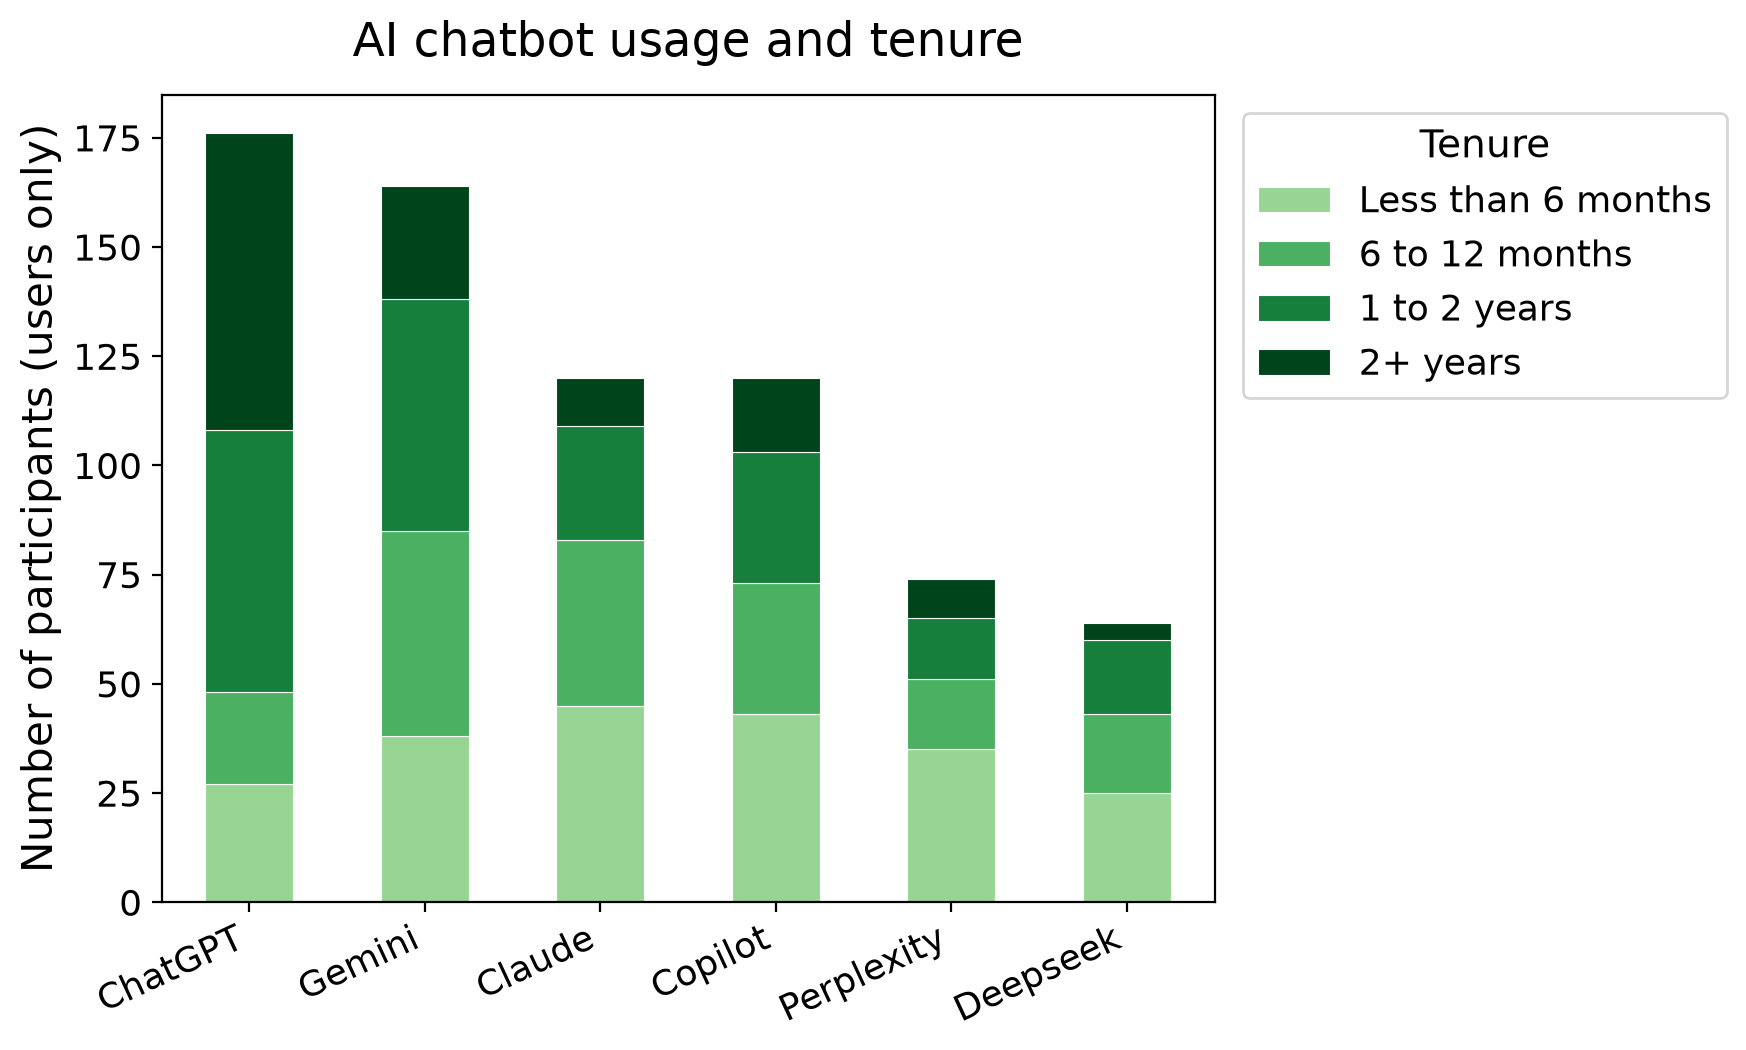
\includegraphics[width=\linewidth]{figures/fig1_ai_tenure.png}
\caption{AI chatbot usage and tenure ($n=177$).}
\label{fig:ai-tenure}
\end{figure}

\subsection{Usage of Data Deletion Methods}
\label{sec:sensitivity-effect}

\textbf{Past use.} Participants had most often used single-conversation deletion (76.8\%), followed by clearing all conversation history (53.1\%), deleting a specific saved memory (32.2\%), asking the chatbot to forget (31.1\%) and clearing all saved memories (25.4\%); account deletion (10.2\%), a privacy dashboard (9.6\%) and filing a request (2.8\%) were rare (Table~\ref{tab:method-usage}). Most had found the options themselves: 42.4\% while browsing the platform settings, 19.8\% by guessing or experimenting, and 19.8\% by searching online or reading documentation. Another 9.0\% were told by someone, and 3.4\% were told or reminded by the platform.

\textbf{Methods chosen in each scenario.} Deleting a single conversation was the most frequent choice in both scenarios (84/177, 47.5\%, in the less-sensitive scenario and 80/177, 45.2\%, in the more-sensitive one), followed by clearing all conversation history (33 and 40 participants; Table~\ref{tab:method-usage}). The distribution of chosen methods did not differ significantly between scenarios (Stuart-Maxwell test, $p=.393$). The more-sensitive scenario was always shown second (\S\ref{sec:survey-methodology}), so every difference between scenarios reported in this section is equally consistent with a sensitivity effect and an order effect.

\textbf{Ideal methods in each scenario.} Participants could mark every method they considered ideal. Deleting a single conversation was again the most often marked (66.1\% and 60.5\%), followed by asking the chatbot to forget (46.9\% and 50.3\%) and clearing all conversation history (35.6\% and 40.7\%) (Table~\ref{tab:method-usage}). No method was marked significantly more or less often in one scenario than in the other after Holm correction across the eight methods (exact McNemar tests). The smallest difference was for deleting a specific saved memory (31.1\% to 41.8\%, $p=.011$, $p_{\mathrm{Holm}}=.088$).

\textbf{Willingness to delete.} Willingness (five-point scale) was higher in the more-sensitive scenario ($M=4.37$) than in the less-sensitive one ($M=3.98$; $\Delta=+0.39$, 95\% CI $[+0.23, +0.55]$, Wilcoxon signed-rank $p<.001$, $r=.55$).

\begin{table*}[t]
\centering
\caption{Deletion methods: past use, method chosen in each scenario, and methods marked ideal in each scenario ($n=177$). ``Other'' was chosen by one participant in each scenario.}
\label{tab:method-usage}
\small
\begin{tabular}{lccccc}
\toprule
 & Ever used & \multicolumn{2}{c}{Chosen, $n$ (\%)} & \multicolumn{2}{c}{Ideal, \%} \\
\cmidrule(lr){3-4}\cmidrule(lr){5-6}
Method & \% & Less & More & Less & More \\
\midrule
Delete a single conversation & 76.8 & 84 (47.5) & 80 (45.2) & 66.1 & 60.5 \\
Clear all conversation history & 53.1 & 33 (18.6) & 40 (22.6) & 35.6 & 40.7 \\
Delete a specific saved memory & 32.2 & 19 (10.7) & 22 (12.4) & 31.1 & 41.8 \\
Ask the chatbot to forget & 31.1 & 25 (14.1) & 14 (7.9) & 46.9 & 50.3 \\
Clear all saved memories & 25.4 & 7 (4.0) & 8 (4.5) & 16.9 & 24.3 \\
Delete the account & 10.2 & 2 (1.1) & 3 (1.7) & 4.5 & 6.2 \\
Privacy dashboard & 9.6 & 6 (3.4) & 9 (5.1) & 15.3 & 17.5 \\
File a request & 2.8 & 0 (0.0) & 0 (0.0) & 2.3 & 5.1 \\
\bottomrule
\end{tabular}
\end{table*}

\subsection{Evaluation of Data Deletion Methods}

Only the four methods chosen by at least 14 participants (single conversation, clear all history, specific memory, ask to forget) enter the tests below; the others are too rare to test. Scale scores are the mean of a scale's items on a five-point agreement scale. Pooled figures use participant-scenario observations ($n=317$ across the four methods), so a participant who chose the same method in both scenarios contributes two.

\subsubsection{Measurement Model}

An exploratory factor analysis of the 12 protection, effort and benefit-loss items (principal axis, oblimin rotation; 354 participant-scenario observations) supported the three intended factors. The sampling was adequate (KMO $=.81$; Bartlett's test $p<.001$), parallel analysis retained three factors (eigenvalues 3.86, 3.58 and 1.86, each above the 95th percentile of random data; the fourth, 0.58, was not), and the three factors explained 70.6\% of the variance. Every item loaded at least .67 on its intended factor and at most .15 on any other (Table~\ref{tab:efa}); the same pattern held within each scenario. Reliability was high for every scale in both scenarios (Cronbach's $\alpha=.87$ to $.92$). The factors were weakly correlated: protection was unrelated to effort ($\rho=-.06$) and to benefit loss ($\rho=.13$), and effort and benefit loss were modestly correlated ($\rho=.31$, $p<.001$).

\begin{table}[t]
\centering
\caption{Factor loadings of the 12 items (pooled observations; signs set so that loadings on the intended factor are positive).}
\label{tab:efa}
\small
\setlength{\tabcolsep}{3pt}
\begin{tabular}{p{0.60\columnwidth}cc}
\toprule
Item & Loading & Largest other \\
\midrule
\multicolumn{3}{l}{\textit{Perceived protection}} \\
Contributes to the protection of my privacy & .83 & .10 \\
Helps me protect my personal information & .86 & .08 \\
Effectively reduces the risk of misuse & .74 & .05 \\
Gives me complete control over my data & .79 & .09 \\
I can decide what the chatbot retains & .79 & .11 \\
\midrule
\multicolumn{3}{l}{\textit{Effort}} \\
Takes too much time & .86 & .03 \\
Is overly complex to use & .94 & .04 \\
Is difficult to navigate & .91 & .03 \\
Understanding it requires significant effort & .75 & .03 \\
\midrule
\multicolumn{3}{l}{\textit{Benefit loss}} \\
Prevents responses tailored to my context & .84 & .03 \\
Reduces relevance of help tailored to me & .96 & .04 \\
Prevents the kind of help I need & .67 & .15 \\
\bottomrule
\end{tabular}
\end{table}

\subsubsection{Perceived Privacy Protection}

Mean protection ratings were similar across methods (pooled means 3.63 to 3.86; Table~\ref{tab:method-scales}), and the methods did not differ significantly: within each scenario Kruskal-Wallis tests found no difference ($p>.15$), and a participant-clustered generalized estimating equation on the pooled observations found none either (Wald $\chi^2(3)=3.71$, $p_{\mathrm{Holm}}=.29$). Scenario-specific means ranged from 3.54 to 3.84 (less-sensitive) and from 3.71 to 3.89 (more-sensitive). Protection was rated higher in the more-sensitive scenario across all participants ($M=3.66$ to $M=3.79$, $\Delta=+0.13$, 95\% CI $[+0.06, +0.21]$, $p<.001$, $r=.38$). Within a method, protection did not differ significantly between the participants who chose it in the less-sensitive scenario and those who chose it in the more-sensitive one (Mann-Whitney tests, all $p_{\mathrm{Holm}}\geq.54$). In a regression on both scenarios' ratings (participant-clustered standard errors), AI literacy was the only participant characteristic associated with protection ($b=0.28$, $p=.016$); age, education, gender and privacy concern were not.

\subsubsection{Benefit Loss}

Mean benefit-loss ratings were highest for deleting a specific saved memory (3.46) and lowest for asking the chatbot to forget (2.91; Table~\ref{tab:method-scales}), but the methods did not differ significantly (within scenarios $p>.15$; pooled Wald $\chi^2(3)=6.94$, $p_{\mathrm{Holm}}=.15$). Benefit loss did not differ between scenarios across all participants ($\Delta=+0.04$, 95\% CI $[-0.07, +0.15]$), nor within any method (Mann-Whitney tests, all $p_{\mathrm{Holm}}=1.00$). No participant characteristic in the regression was associated with benefit loss (all $p\geq.10$).

\subsubsection{Effort}

Effort was the only rating on which methods differed (pooled Wald $\chi^2(3)=23.05$, $p_{\mathrm{Holm}}<.001$; less-sensitive $H=18.42$, $p<.001$; more-sensitive $H=16.98$, $p<.001$). Deleting a single conversation had the lowest mean (1.64) and deleting a specific saved memory the highest (2.49; Table~\ref{tab:method-scales}). In pooled contrasts, participants who chose single-conversation deletion reported lower effort than those who chose specific-memory deletion (mean difference $-0.85$, 95\% CI $[-1.25, -0.46]$, $p_{\mathrm{Holm}}<.001$) and than those who chose clear-all-history ($-0.45$, $[-0.76, -0.14]$, $p_{\mathrm{Holm}}=.019$), but not lower than those who asked the chatbot to forget ($-0.10$, $[-0.39, +0.19]$); asking to forget was also rated lower than specific-memory deletion ($-0.75$, $[-1.22, -0.29]$, $p_{\mathrm{Holm}}=.008$). Within scenarios, only single-conversation versus specific-memory deletion in the less-sensitive scenario was significant ($p_{\mathrm{Holm}}<.001$). Method choice was self-selected, so these are associations with the chosen method, not effects of switching methods. Effort did not differ between scenarios across all participants ($\Delta=+0.03$, 95\% CI $[-0.06, +0.12]$), nor within any method (Mann-Whitney tests, all $p_{\mathrm{Holm}}=1.00$). Higher AI literacy was associated with lower effort ($b=-0.29$, $p=.008$); the other characteristics were not.

\begin{table*}[t]
\centering
\caption{Mean (SD) protection, benefit loss and effort by chosen deletion method, pooled and by scenario. $n$ is the number of observations (pooled; less-sensitive; more-sensitive).}
\label{tab:method-scales}
\small
\setlength{\tabcolsep}{4pt}
\begin{tabular}{lcccccccccc}
\toprule
 & & \multicolumn{3}{c}{Protection} & \multicolumn{3}{c}{Benefit loss} & \multicolumn{3}{c}{Effort} \\
\cmidrule(lr){3-5}\cmidrule(lr){6-8}\cmidrule(lr){9-11}
Method & $n$ & Pooled & Less & More & Pooled & Less & More & Pooled & Less & More \\
\midrule
Single conversation & 164; 84; 80 & 3.63 (0.88) & 3.54 & 3.73 & 3.00 (1.03) & 2.97 & 3.02 & 1.64 (0.76) & 1.62 & 1.67 \\
Clear all history & 73; 33; 40 & 3.77 (0.87) & 3.77 & 3.77 & 3.11 (1.10) & 3.06 & 3.14 & 2.09 (0.97) & 1.98 & 2.18 \\
Specific memory & 41; 19; 22 & 3.65 (0.79) & 3.58 & 3.71 & 3.46 (0.88) & 3.54 & 3.38 & 2.49 (1.03) & 2.70 & 2.32 \\
Ask to forget & 39; 25; 14 & 3.86 (0.65) & 3.84 & 3.89 & 2.91 (0.95) & 2.91 & 2.90 & 1.74 (0.79) & 1.86 & 1.54 \\
\bottomrule
\end{tabular}
\end{table*}

\subsubsection{Expectations of Data Deletion Methods}

\textbf{Expected outcomes.} Across both scenarios, participants most often expected the data to be permanently deleted from the chatbot's database and backups (59.0\% of observations), followed by the chatbot no longer referencing it in future conversations (54.2\%) or in the current one (49.2\%); 28.5\% expected it to be hidden from users, 27.7\% expected it to be excluded from training, and 10.5\% were unsure. Expectations did not differ significantly by method (Table~\ref{tab:contingency}; participant-clustered GEE for each option, Holm-corrected across seven options, all $p_{\mathrm{Holm}}\geq.37$; Cram\'er's $V\leq.18$). The observed rates differed by up to 29 percentage points for some options, so this is a failure to detect an association at these group sizes, not evidence that methods elicit the same expectations.

\textbf{Verification.} The most common verification response was not knowing how to check (46.7\% of observations), followed by asking in the same conversation (20.5\%), asking in a new conversation (19.2\%), checking the interface (15.8\%) and checking the settings (14.5\%); 11.4\% did not want to check (Table~\ref{tab:verification}). Verification differed by method. In the less-sensitive scenario, method was associated with asking in the same conversation ($p_{\mathrm{Holm}}=.001$), asking in a new conversation ($p_{\mathrm{Holm}}=.007$) and not knowing how to verify ($p_{\mathrm{Holm}}=.007$); in the more-sensitive scenario, with asking in the same conversation ($p_{\mathrm{Holm}}=.039$) and checking the settings ($p_{\mathrm{Holm}}=.046$). Those who chose the lowest-effort method, single-conversation deletion, most often did not know how to verify (58.5\%).

\textbf{Deleted information referenced again.} Nearly a quarter (23.7\%) had noticed a chatbot referencing information they believed they had deleted (20.3\% occasionally, 3.4\% frequently); 49.2\% had never noticed this, 24.3\% were not sure, and 2.8\% had never attempted deletion.

\textbf{Post-deletion feedback.} Currently, 41.2\% received a clear message confirming deletion, 34.5\% a brief or vague acknowledgement, and 29.4\% no feedback. Participants most often wanted a popup confirmation (68.4\%) or a breakdown of what was deleted and what may be retained (41.2\%), followed by a timestamp or estimate of when deletion completes (27.7\%), an inline confirmation in the conversation (23.7\%) and an email (22.6\%); 8.5\% wanted no feedback.

\begin{table}[t]
\centering
\caption{Deletion Method $\times$ Expectation (Pooled Participant-Scenario
Observations), \% of Each Method's Observations}
\label{tab:contingency}
\small
\setlength{\tabcolsep}{3pt}
\begin{tabular}{lcccc}
\toprule
Method (obs.) & Perm. & Not ref. & Not ref. & No longer \\
 & deleted & (current) & (future) & trained \\
\midrule
Single conv. (164)  & 58.5 & 44.5 & 54.3 & 28.0 \\
Clear history (73)  & 52.1 & 39.7 & 42.5 & 16.4 \\
Specific memory (41) & 65.9 & 68.3 & 63.4 & 19.5 \\
``Forget'' msg (39) & 64.1 & 53.8 & 51.3 & 35.9 \\
\bottomrule
\end{tabular}
\end{table}

\begin{table*}[t]
\centering
\caption{Deletion Method $\times$ Verification (Pooled Participant-Scenario
Observations), \% of Each Method's Observations}
\label{tab:verification}
\small
\setlength{\tabcolsep}{4pt}
\begin{tabular}{lccccccc}
\toprule
Method (obs.) & Asked, same & Asked, new & Checked & Checked & Privacy & Did not & Did not \\
 & conv. & conv. & settings & interface & portal & know how & want to \\
\midrule
Single conv. (164)  & 12.8 & 12.8 & 10.4 & 14.6 & 2.4 & 58.5 & 12.2 \\
Clear history (73)  & 19.2 & 17.8 & 13.7 & 23.3 & 6.8 & 42.5 & 11.0 \\
Specific memory (41) & 22.0 & 34.1 & 36.6 & 12.2 & 2.4 & 29.3 & 12.2 \\
``Forget'' msg (39) & 53.8 & 33.3 & 10.3 & 10.3 & 0.0 & 23.1 & 7.7 \\
\midrule
All (317) & 20.5 & 19.2 & 14.5 & 15.8 & 3.2 & 46.7 & 11.4 \\
\bottomrule
\end{tabular}
\end{table*}

\section{Technical Audit Results}
\label{sec:audit-results}
% TODO(authors): drives RQ1 (observed deletion-control behavior per
% platform/cell, recorded as the four measurements described under
% "Outcome recording and repetition" in \S\ref{sec:audit-methodology}),
% RQ2 (where observed behavior contradicts each platform's documented
% commitment; "Policy commitments" and Table~\ref{tab:consistency-rule} in
% \S\ref{sec:audit-methodology} give the exact contradiction rule; report
% the counts of each commitment type so readers can see how many cells
% could support a verdict at all, and report mismatches between
% acknowledgment and state as their own finding), and, together with
% \S\ref{sec:sample-knowledge} and \S\ref{sec:sensitivity-effect}, feeds
% RQ5 (Discussion) once real per-cell outcome data exists to report. For
% RQ5 specifically: map each survey expectation option to the specific
% platform/control/surface combination it could in principle be checked
% against (sharing six platform names across survey and audit does not by
% itself make them matched), and keep two kinds of finding visibly
% distinct rather than merging them into one "gap" number: (a) an
% observable mismatch, where the audit's documented commitment
% for a cell contradicts what participants expected, both anchored to a
% specific platform/control; and (b) an expectation this audit's
% measurement scope (\S\ref{sec:audit-methodology}'s
% "Measurement scope") cannot verify either way (chiefly training-data
% exclusion), which is a scope limitation to report, not a confirmed
% mismatch. "Who bears that gap" needs a stated subgroup (e.g., by method
% choice or by platform) or should be narrowed to whichever comparison the
% data actually support. Draft from the Acknowledgment and Interface change
% columns, the recall columns and the commitment types in MASTER, FILE
% SUBSTUDY and NL FORGET (Recoverability and Policy consistency are
% computed from them), and tester/transcripts/, once the
% audit reaches a reportable stopping point (either full completion or a
% pre-registered interim cut), not before; do not draft this from
% partial/in-progress data presented as final.
TBWL

\section{Discussion}
\label{sec:discussion}

\textbf{Training-data exclusion is a distinct technical problem from record
deletion.} Deletion that removes a record does not, by itself, remove
that record's influence on a model already trained on it; machine-unlearning
research treats this as a distinct, harder problem than record-level
deletion~\cite{bourtoule2021machine}. In the survey, most participants
selected ``permanently deleted'' as an expected outcome, while only 15--36\%
(depending on the method chosen) also selected ``no longer used for training the AI model''
(\S\ref{sec:sample-knowledge}). This selection pattern does not show that
participants conflate the two outcomes. The item was select-all, so leaving an
option unselected does not mean a participant believes its opposite. The
``permanently deleted'' option was worded as deletion ``from the database and
backups,'' a claim about stored copies, so a participant may have read it as
applying to the surface they acted on and said nothing about training.
Participants may also have been unsure about training, or judged that option
redundant or unclear as worded. The training option itself did not separate
preventing future training use from removing the influence of data already
used in training, which are different expectations. We therefore report the
selection pattern without inferring a misconception; distinguishing these
readings would take explicit questions, open-ended explanations, or
interviews. Whether the expectations participants did select match what
today's chatbot deletion controls guarantee is a question the technical
audit (RQ2/RQ5) takes up directly.

\textbf{Low verification is a recurring failure mode, not a new one.}
Usable-privacy work on other deletion surfaces has repeatedly found that
a deletion control's existence does not guarantee it is understood,
locatable, or actually checked. This holds for cloud-storage
deletion~\cite{ramokapane2017stupid} and for website data-deletion and
opt-out controls audited directly~\cite{habib2019empirical}.
Participants' self-reported verification behavior fits the same pattern
in a new setting: nearly half (46.7\% of observations) did not know how
to check whether a chatbot deletion worked (\S\ref{sec:sample-knowledge}). These are participants' recollections of
past behavior on the survey's verification item, not actions the study
observed directly, a distinction the technical audit's own recall probes
(\S\ref{sec:audit-methodology}) are designed to check independently. With
that caveat, the pattern suggests the verification gap is a property of
how deletion controls are generally designed and explained, not something
specific to any one platform's implementation.

\textbf{The memory-deletion cost matches a known mental-model gap.}
Interview work on LLM chatbot memory features finds that users hold
diverse, often incomplete models of what a stored ``memory'' represents
and how it was formed, and want finer-grained control over
it~\cite{zhang2025understanding}. That gives a plausible mechanism for
this paper's own finding that ``delete a specific saved memory'' is both
the highest-effort and highest-benefit-loss method participants
rated (\S\ref{sec:sample-knowledge}): if a user is unsure what a memory
entry represents or how it was derived, deciding whether and how to
delete it is harder than deleting a single conversation turn, independent
of how many clicks either action actually takes.

\textbf{Willingness to delete was higher when the data were more sensitive,
and the controls available to act on it are uneven.} Willingness to delete and
perceived protection were both higher in the more-sensitive scenario
(\S\ref{sec:survey-methodology} notes this is confounded with presentation
order). Li et al.'s
walkthrough finds that LLM platforms' deletion controls are already
inconsistently implemented across accounts and message types~\cite{li2026privacy}.
Whether the controls users can reach keep pace with their willingness to
delete is a question this paper's user-side data cannot settle alone: it would
require separating control availability, control discoverability, and user
effort tolerance.

\textbf{Design implications.} Across the points above, the survey's selection
patterns are consistent with participants expecting deletion to reach stored
copies (most selected permanent deletion), with training exclusion being a
less frequently selected outcome, and with limited knowledge of how to verify
a deletion (about 45\% did not know how). These are implications drawn from
association patterns in self-reported data, not interventions this study
evaluated. If the patterns hold, a chatbot platform that wants its deletion
controls to function as a right-to-erasure mechanism, rather than a
lightweight convenience action, could address both by stating plainly what a
given control does and does not remove and by making the outcome possible to
confirm. Whether either change alters what users understand or do would need
to be tested directly, and the mismatch RQ5 measures would remain for
whichever of the two was left unaddressed.

\section{Limitations}
\label{sec:limitations}
% TODO(authors): survey-side limitations: the two scenarios were shown in a
% fixed, non-counterbalanced order (\S\ref{sec:survey-methodology}), so
% every sensitivity comparison in \S\ref{sec:sensitivity-effect} is equally
% consistent with an order effect and cannot isolate sensitivity as the
% cause; sample skew (young, US-only, high baseline privacy knowledge,
% \S\ref{sec:sample-knowledge}); the eligibility screen excludes people who
% never deleted chatbot data (36 of 218; see Sample scope in
% \S\ref{sec:survey-methodology}), so results say nothing about those who
% never found a deletion control; pooled analyses treat a participant's two
% scenario responses as clustered, not independent; self-report of past deletion
% behavior/expectations, underpowered
% subgroup tests (McNemar per-method power caveats noted in the results,
% e.g. \S~B9/global.md). Technical-audit-side limitations (once its
% Results are drafted), e.g. all 6 test accounts are free/no-cost tier
% (Perplexity's Memory feature, and everything depending on it, is
% inaccessible on that tier, a real access finding, not just a testing
% gap, but still worth naming as a scope limitation here too), accounts
% reused across cells with contamination controlled via unique per-cell
% anchor+token rather than fresh-account isolation, acknowledgment
% recorded from a single observation per cell since there is no safe way
% to re-request the same erasure (recall's own outcome-dependent-
% repetition asymmetry was fixed 2026-09-23 with a mandatory two-attempt
% policy -- see "Outcome recording and repetition" in
% \S\ref{sec:audit-methodology} -- so this residual limitation is scoped
% to the acknowledgment measurement only, not recall), retention is read
% from the platform's own reply and interface status at injection, not
% from control cells (see "Retention at injection" in
% \S\ref{sec:audit-methodology}), so cells with no such signal, most of
% them on Gemini, DeepSeek and Perplexity, stay indeterminate, a status or
% a claim is not proof that the fact sits on a memory surface, and change
% over the 31-day window is not tested, and
% platform UI changes during the study window (e.g. ChatGPT's memory
% redesign removing per-item deletion mid-study; Copilot's move to
% copilot.com, disclosed under "Platform changes" in
% \S\ref{sec:audit-methodology}, which puts its recall on a different
% interface from injection) limiting how directly
% results generalize forward in time. Also from the outcome coding:
% acknowledgment shows what a platform said, not what it stored;
% commitment types rest on the platforms' published documentation as
% read during the audit and can change; NO COMMITMENT, UNRELATED and NOT
% TESTABLE cells cannot support a verdict on policy; the ChatGPT and
% Perplexity help pages returned HTTP 403 to direct fetch, so their
% commitment wording was copied by hand from the live pages on
% 2026-09-24 (the pages are revised often: the ChatGPT ones were updated
% within days of that date, so the wording is dated, not permanent); and acknowledgment for chat-based
% erasure requests was read from screenshots by optical character
% recognition, with replies that were cut off, covered or not yet
% displayed reported as not captured.
TBWL

\section{Conclusion}
% TODO(authors): 1-2 paragraphs restating the core contribution and
% takeaway without re-deriving statistics already given in Results.
TBWL

% ----------------------------------------------------------------
\section*{Ethics Considerations}
% Required disclosure per the IEEE S&P 2027 CFP for work involving
% human-subjects data. Fill in the bracketed items before submission --
% do not leave placeholders in the submitted PDF. This section is also
% requested as a separate field on HotCRP at registration; keep the two
% consistent. At camera-ready this section is added/finalized without
% counting against the page limit, but reviewers see whatever is here
% at submission time, so complete it now rather than deferring it.
% Anonymous submission: institution name and IRB ID withheld; restore at
% camera-ready (University of Central Florida IRB, MOD00008224).
The survey was reviewed by the authors' institutional review board, which
determined on 2026-06-25 that it is human subjects research exempt from
regulation (exemption categories 2.i and 3A). Participants were recruited through Prolific, were
US-resident adults who had used at least one of the six chatbots, and
consented on the first page of the survey before any question; declining
ended the survey. Participation was voluntary and paid \$4 through
Prolific on completing the survey and passing the attention checks. The
survey was anonymous: no name, email address or other identifying
information was collected, responses were stored on access-restricted
university storage, and study records are kept for at least five years after
study closure. The consent form stated that de-identified data may be used
in future research or academic publications without additional consent.
Two attention and eligibility checks (failed the attention check; had never
deleted chatbot data before) were applied before the quantitative survey
analysis, excluding 37 of 218 complete responses
(\S\ref{sec:sample-knowledge}), so those analyses use only eligible,
attentive respondents' data. The deletion-request prompt corpus
(\S\ref{sec:prompt-corpus}) is built differently: it includes the prompt
text of every respondent who wrote one, whether or not that respondent later
passed these checks (209 authors, 375 distinct prompts), because the prompts
serve as realistic phrasings for the audit, not as survey measurements.
Consent was required to enter the survey, so excluded respondents gave it
under the same form as included ones. Before the prompts were used in the
audit, residual personally identifying text was redacted (\S\ref{sec:prompt-corpus}).

The technical audit (RQ1, RQ2, RQ5) interacted with six commercial LLM
chatbot platforms (Claude, ChatGPT, Gemini, Copilot, Perplexity,
DeepSeek) using researcher-controlled accounts created for this study,
not third-party or compromised accounts. Every action (sending messages,
uploading documents, invoking each platform's own memory, settings, and
deletion controls) used standard, publicly available account
functionality that an ordinary logged-in user could perform manually; no
vulnerability was exploited, no authentication or authorization boundary
was bypassed, and no other user's data was accessed at any point.
Two of the six platforms additionally required routing browser automation
through \texttt{playwright-stealth} to complete a session: without it,
generic bot-fingerprinting checks (Cloudflare) blocked the automated
browser from an already-authenticated account before it could perform
any action at all, including ones a human operator of that same account
could perform unmodified. This defeats a bot-detection heuristic aimed at
traffic patterns, not an access-control mechanism gating who may act on
the account: the stealth plugin changes how the browser presents itself,
not what credentials or authorization it holds, and every action taken
after a session loaded was identical in kind to a manual one. Potential
harm is confined to the researchers' own test-account data; the study
does not disrupt other users, access confidential information, or alter
shared infrastructure. We did not seek permission from the platforms: all
six accounts were free-tier accounts, and every action was available to any
free-tier user. The IRB review covered the survey only; the audit involved
no human subjects beyond the use of the redacted survey prompts described above.
We see no path to harm for any person: the audit used only our own accounts,
accessed no other user's data, and sent ordinary requests through each
platform's public interface. Its benefit is direct evidence on whether the
deletion controls users rely on do what platforms say they do, which users
cannot currently verify for themselves.

\appendix

\section{Survey Instrument}
\label{sec:instrument}

\textbf{Scenarios.} Each scenario opened with the text ``Imagine that you
are chatting with an AI chatbot\ldots'' followed by the conversation
below and the instruction to delete the data disclosed in it.

\begin{itemize}[leftmargin=*,nosep]
\item \textit{Less sensitive (weather).} User: ``I am in Orlando now.
What's the weather today in Orlando?'' AI: ``Based on your city, it's
72\,$^{\circ}$F and sunny. There is a slight chance of rain this
evening.'' User: ``Should I bring an umbrella?'' AI: ``Probably not. The
chance of rain is only 10\%.'' \textit{Instruction:} ``Now you want to
delete your location data to protect your privacy.''
\item \textit{More sensitive (health).} User: ``I live at 7482 Orange
Blossom Lane, Orlando, FL 32801. Can you find me the nearest Medical
Center to get treatment for sexually transmitted infections?'' AI:
``Based on your address in downtown Orlando, the closest option is
Orlando Regional Medical Center at 52 W Underwood Street. If it's a
life-threatening emergency, call 911 rather than driving yourself.''
User: ``How should I prepare?'' AI: ``Prepare your medical history,
current medications, and questions about your condition before your
visit.'' \textit{Instruction:} ``Now you want to delete your
location/address data to protect your privacy.''
\end{itemize}

\textbf{Scales.} In each scenario, respondents rated the deletion method
they chose on a five-point agreement scale (Strongly Disagree,
Disagree, Neutral, Agree, Strongly Agree). The three scales, with their
items, are:

\begin{itemize}[leftmargin=*,nosep]
\item \textit{Perceived protection} (5 items): ``This data deletion method
contributes to the protection of my privacy''; ``\ldots helps me to
protect my personal information''; ``\ldots effectively reduces the risk
of my data being misused''; ``\ldots gives me complete control over my
personal data''; ``By using this data deletion method, I can decide what
personal data the AI Chatbot retains about me.''
\item \textit{Effort} (4 items): ``This data deletion method takes too
much time''; ``\ldots is overly complex to use''; ``I find it difficult to
navigate this data deletion method''; ``Understanding how this data
deletion method works requires significant effort.''
\item \textit{Benefit loss} (3 items): ``Using this data deletion method
would prevent AI Chatbots from providing responses tailored to my
activity context''; ``\ldots would reduce the relevance of assistance
tailored to my preferences''; ``Using this data deletion feature would
prevent AI Chatbots from providing the kind of help I need.''
\end{itemize}

\textbf{Attention checks.} ``Please select `Sometimes' for this question''
(frequency scale from Never to Always) and ``Please select `Agree' for
this question'' (agreement scale).

% ----------------------------------------------------------------
% TODO(authors): populate refs.bib further as the Background/Related
% Work literature review is written (a GDPR Art. 17 entry is already
% in refs.bib so \cite{gdpr2016} above resolves). IEEEtran bibliography
% style is required by the CFP template; do not substitute another.
\bibliographystyle{IEEEtran}
\bibliography{refs}


\end{document}
